\documentclass[11pt]{article}

% --- Packages ---
\usepackage[margin=0.9in]{geometry}
\usepackage{amsmath,amssymb,amsfonts}
\usepackage{graphicx}
\usepackage{tikz}
\usepackage{enumitem}
\usepackage{xcolor}
\usepackage{tcolorbox}
\usepackage{fancyhdr}
\usepackage{cancel}
\tcbuselibrary{breakable,skins}

% --- Header ---
\pagestyle{fancy}
\fancyhf{}
\lhead{\textbf{Algebra 2 \textbullet{} Lesson 4-3}}
\rhead{Worked Examples 1--6}
\cfoot{\thepage}

% --- Environments ---
\newtcolorbox{example}[1]{
  colback=blue!3!white,
  colframe=blue!55!black,
  fonttitle=\bfseries,
  title={#1},
  breakable,
  enhanced
}

\newtcolorbox{tryit}{
  colback=yellow!8!white,
  colframe=orange!70!black,
  fonttitle=\bfseries,
  title={Try It!},
  breakable,
  enhanced
}

\newtcolorbox{annot}{
  colback=gray!8!white,
  colframe=gray!50!black,
  arc=2mm,
  boxsep=2pt,
  left=4pt, right=4pt, top=2pt, bottom=2pt
}

\newcommand{\workspace}[1]{\vspace{#1}}
\newcommand{\domain}[1]{\text{Domain: } #1}

\title{\textbf{Lesson 4-3: Worked Examples} \\ \large Multiplying and Dividing Rational Expressions}
\author{}
\date{}

\begin{document}

\maketitle
\vspace{-2em}

% ====================================================================
% EXAMPLE 1
% ====================================================================
\begin{example}{Example 1 --- Write Equivalent Rational Expressions}
Write an expression equivalent to $\dfrac{x+3}{x+9}$. For what domain are the expressions equivalent?

\vspace{0.5em}
\textit{Strategy:} Multiply by factors equal to $1$ to produce an equivalent rational expression. Here, use $\dfrac{x-6}{x-6}$ and $\dfrac{x}{x}$.

\begin{align*}
\dfrac{x+3}{x+9} &= \dfrac{x+3}{x+9}\cdot 1 \cdot 1 \\[4pt]
&= \dfrac{x+3}{x+9}\cdot \dfrac{x-6}{x-6}\cdot \dfrac{x}{x} \\[4pt]
&= \dfrac{(x+3)(x-6)x}{(x+9)(x-6)x} \\[4pt]
&= \dfrac{x^{3}-3x^{2}-18x}{x^{3}+3x^{2}-54x}
\end{align*}

\begin{annot}
Since $x^{3}+3x^{2}-54x = x(x+9)(x-6)$, the new expression is undefined at $x=0$, $x=-9$, and $x=6$. Those values must be excluded from the domain.
\end{annot}

The two forms are equal on the intersection of their domains. So
\[
\dfrac{x+3}{x+9} \;=\; \dfrac{x^{3}-3x^{2}-18x}{x^{3}+3x^{2}-54x} \quad \text{for } \{x \mid x \in \mathbb{R},\ x \neq 0,\ 6,\ -9\}.
\]
\end{example}

\begin{tryit}
\textbf{1.} Write an expression equivalent to $\dfrac{x-4}{x}$ over the domain $\{x \mid x \neq 0 \text{ or } -2\}$.
\workspace{4cm}
\end{tryit}

\newpage

% ====================================================================
% EXAMPLE 2
% ====================================================================
\begin{example}{Example 2 --- Simplify a Rational Expression}
Simplify the rational expression, and state the domain on which the identity holds:
\[
\dfrac{4-x^{2}}{x^{2}+3x-10}
\]

\vspace{0.5em}
\textit{Strategy:} A rational expression is in \textbf{simplified form} when the numerator and denominator share no common factors other than $1$. Factor first, then cancel.

\begin{align*}
\dfrac{4-x^{2}}{x^{2}+3x-10} &= \dfrac{(2-x)(2+x)}{(x-2)(x+5)} \\[6pt]
&= \dfrac{-(x-2)(x+2)}{(x-2)(x+5)} \qquad \text{since } 2-x = -(x-2)\\[6pt]
&= -\,\dfrac{\cancel{(x-2)}(x+2)}{\cancel{(x-2)}(x+5)} \\[6pt]
&= -\,\dfrac{x+2}{x+5}
\end{align*}

\begin{annot}
\textbf{Common Error.} The factor $(2-x)$ does not look identical to $(x-2)$, but $2-x = -1\cdot(x-2)$. Always check for sign-flipped common factors before declaring two polynomials have no factor in common.
\end{annot}

\[
\dfrac{4-x^{2}}{x^{2}+3x-10} \;=\; -\dfrac{x+2}{x+5}, \qquad x \neq 2 \text{ or } -5.
\]
\end{example}

\begin{tryit}
\textbf{2.} Simplify each expression and state the domain.

\vspace{0.3em}
\begin{minipage}[t]{0.48\textwidth}
\textbf{a.} $\dfrac{x^{2}+2x+1}{x^{3}-2x^{2}-3x}$
\workspace{3.5cm}
\end{minipage}\hfill
\begin{minipage}[t]{0.48\textwidth}
\textbf{b.} $\dfrac{x^{3}+4x^{2}-x-4}{x^{2}+3x-4}$
\workspace{3.5cm}
\end{minipage}
\end{tryit}

\newpage

% ====================================================================
% EXAMPLE 3
% ====================================================================
\begin{example}{Example 3 --- Multiply Rational Expressions}
\textbf{A.} What is the product of $\dfrac{2xy}{z}$ and $\dfrac{3x^{2}}{4yz}$?

\vspace{0.4em}
Multiply numerators and denominators just as you would with numerical fractions, then cancel common factors.
\begin{align*}
\dfrac{2xy}{z}\cdot \dfrac{3x^{2}}{4yz} &= \dfrac{(2xy)(3x^{2})}{z(4yz)} \\[4pt]
&= \dfrac{\cancel{2}\cdot 3 \cdot \cancel{y}\cdot x \cdot x^{2}}{\cancel{2}\cdot 2 \cdot \cancel{y}\cdot z \cdot z^{2}} \\[4pt]
&= \dfrac{3x^{3}}{2z^{2}}, \qquad y \neq 0,\ z \neq 0
\end{align*}

\vspace{0.5em}
\hrule
\vspace{0.5em}

\textbf{B.} Find the product in simplified form:
\[
\dfrac{5x}{x+3}\cdot \dfrac{x^{2}+x-6}{x^{2}+2x+1}\cdot \dfrac{x^{2}+x}{5x-10}
\]

\vspace{0.3em}
Factor everything, then identify common factors.
\begin{align*}
&\dfrac{5x}{x+3}\cdot \dfrac{x^{2}+x-6}{x^{2}+2x+1}\cdot \dfrac{x^{2}+x}{5x-10} \\[4pt]
&\qquad = \dfrac{5x(x+3)(x-2)\,x(x+1)}{(x+3)(x+1)(x+1)\cdot 5(x-2)} \\[6pt]
&\qquad = \dfrac{\cancel{5}x\cancel{(x+3)}\cancel{(x-2)}\,x\cancel{(x+1)}}{\cancel{5}\cancel{(x+3)}(x+1)\cancel{(x+1)}\cancel{(x-2)}} \\[6pt]
&\qquad = \dfrac{x^{2}}{x+1}
\end{align*}

\[
\dfrac{5x}{x+3}\cdot \dfrac{x^{2}+x-6}{x^{2}+2x+1}\cdot \dfrac{x^{2}+x}{5x-10} \;=\; \dfrac{x^{2}}{x+1}, \qquad x \neq -3,\ -1,\ \text{or } 2.
\]

\begin{annot}
\textbf{Use Structure.} The product of any two rational expressions is itself a rational expression. This is one piece of evidence that rational expressions are \emph{closed} under multiplication.
\end{annot}
\end{example}

\begin{tryit}
\textbf{3.} Find the simplified form of each product, and state the domain.

\vspace{0.3em}
\begin{minipage}[t]{0.48\textwidth}
\textbf{a.} $\dfrac{x^{2}-16}{9-x}\cdot \dfrac{x^{2}+x-90}{x^{2}+14x+40}$
\workspace{3.5cm}
\end{minipage}\hfill
\begin{minipage}[t]{0.48\textwidth}
\textbf{b.} $\dfrac{x+3}{4x}\cdot \dfrac{3x-18}{6x+18}\cdot \dfrac{x^{2}}{4x+12}$
\workspace{3.5cm}
\end{minipage}
\end{tryit}

\newpage

% ====================================================================
% EXAMPLE 4
% ====================================================================
\begin{example}{Example 4 --- Multiply a Rational Expression by a Polynomial}
Find the product of $\dfrac{x+2}{x^{4}-16}$ and $x^{3}+4x^{2}-12x$.

\vspace{0.4em}
\textit{Strategy:} Write the polynomial as a rational expression with denominator $1$. This makes it easier to track positions of factors when canceling.

\begin{align*}
\dfrac{x+2}{x^{4}-16}\cdot (x^{3}+4x^{2}-12x) &= \dfrac{x+2}{x^{4}-16}\cdot \dfrac{x^{3}+4x^{2}-12x}{1} \\[4pt]
&= \dfrac{(x+2)\,x(x^{2}+4x-12)}{1\cdot (x^{2}+4)(x^{2}-4)} \\[4pt]
&= \dfrac{(x+2)\,x(x+6)(x-2)}{(x^{2}+4)(x+2)(x-2)} \\[4pt]
&= \dfrac{\cancel{(x+2)}\,x(x+6)\cancel{(x-2)}}{(x^{2}+4)\cancel{(x+2)}\cancel{(x-2)}} \\[4pt]
&= \dfrac{x(x+6)}{x^{2}+4}
\end{align*}

\begin{annot}
\textbf{Common Error.} Only common \emph{factors} cancel, not common \emph{terms}. You cannot cancel an $x$ out of $\dfrac{x}{x^{2}+4}$ --- the $x^{2}+4$ in the denominator is a sum, not a product involving $x$.
\end{annot}

\[
\dfrac{x+2}{x^{4}-16}\cdot (x^{3}+4x^{2}-12x) \;=\; \dfrac{x(x+6)}{x^{2}+4}, \qquad x \neq -2 \text{ or } 2.
\]
\end{example}

\begin{tryit}
\textbf{4.} Find the simplified form of each product, and state the domain.

\vspace{0.3em}
\begin{minipage}[t]{0.48\textwidth}
\textbf{a.} $\dfrac{x^{3}-4x}{6x^{2}-13x-5}\cdot (2x^{3}-3x^{2}-5x)$
\workspace{3.8cm}
\end{minipage}\hfill
\begin{minipage}[t]{0.48\textwidth}
\textbf{b.} $\dfrac{3x^{2}+6x}{x^{2}-49}\cdot (x^{2}+9x+14)$
\workspace{3.8cm}
\end{minipage}
\end{tryit}

\newpage

% ====================================================================
% EXAMPLE 5
% ====================================================================
\begin{example}{Example 5 --- Divide Rational Expressions}
Find the quotient of $\dfrac{x^{3}+3x^{2}+3x+1}{1-x^{2}}$ and $\dfrac{x^{2}+5x+4}{x^{2}+3x-4}$.

\vspace{0.4em}
\textit{Strategy:} Division by a rational expression is multiplication by its reciprocal.

\begin{align*}
&\dfrac{x^{3}+3x^{2}+3x+1}{1-x^{2}}\;\div\;\dfrac{x^{2}+5x+4}{x^{2}+3x-4} \\[6pt]
&\qquad = \dfrac{x^{3}+3x^{2}+3x+1}{1-x^{2}}\cdot \dfrac{x^{2}+3x-4}{x^{2}+5x+4} \\[6pt]
&\qquad = \dfrac{(x+1)(x+1)(x+1)\cdot (x+4)(x-1)}{-(x-1)(x+1)\cdot (x+1)(x+4)} \\[6pt]
&\qquad = \dfrac{(x+1)}{-1}\cdot \dfrac{\cancel{(x+1)}}{\cancel{(x+1)}}\cdot \dfrac{\cancel{(x+1)}}{\cancel{(x+1)}}\cdot \dfrac{\cancel{(x-1)}}{\cancel{(x-1)}}\cdot \dfrac{\cancel{(x+4)}}{\cancel{(x+4)}} \\[6pt]
&\qquad = -(x+1)
\end{align*}

\begin{annot}
\textbf{Use Structure.} This problem can also be written as a complex fraction:
\[
\dfrac{\;\;\dfrac{x^{3}+3x^{2}+3x+1}{1-x^{2}}\;\;}{\;\;\dfrac{x^{2}+5x+4}{x^{2}+3x-4}\;\;}
\]
Any complex fraction can be rewritten as a division statement.
\end{annot}

\[
\dfrac{x^{3}+3x^{2}+3x+1}{1-x^{2}} \;\div\; \dfrac{x^{2}+5x+4}{x^{2}+3x-4} \;=\; -(x+1), \qquad x \neq -4,\ -1,\ \text{or } 1.
\]
\end{example}

\begin{tryit}
\textbf{5.} Find the simplified quotient and the domain of each expression.

\vspace{0.3em}
\begin{minipage}[t]{0.48\textwidth}
\textbf{a.} $\dfrac{1}{x^{2}+9x}\;\div\;\dfrac{6-x}{3x^{2}-18x}$
\workspace{3.8cm}
\end{minipage}\hfill
\begin{minipage}[t]{0.48\textwidth}
\textbf{b.} $\dfrac{2x^{2}-12x}{x+5}\;\div\;\left(\dfrac{x-6}{x+5}\right)$
\workspace{3.8cm}
\end{minipage}
\end{tryit}

\newpage

% ====================================================================
% EXAMPLE 6
% ====================================================================
\begin{example}{Example 6 --- Use Division of Rational Expressions (Application)}
A company is evaluating two packaging options. The more efficient design will have the smaller ratio of surface area to volume. Should the company use a cube-shaped box or a cylinder?

\vspace{0.5em}
\begin{center}
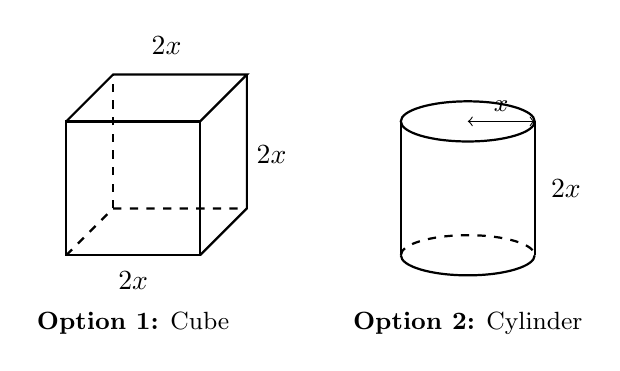
\begin{tikzpicture}[scale=0.85]
  % Cube of side 2x
  \begin{scope}[shift={(0,0)}]
    \draw[thick] (0,0) rectangle (2,2);
    \draw[thick] (0,2) -- (0.7,2.7) -- (2.7,2.7) -- (2,2);
    \draw[thick] (2,0) -- (2.7,0.7) -- (2.7,2.7);
    \draw[thick,dashed] (0,0) -- (0.7,0.7) -- (2.7,0.7);
    \draw[thick,dashed] (0.7,0.7) -- (0.7,2.7);
    \node[below] at (1,-0.1) {$2x$};
    \node[right] at (2.7,1.5) {$2x$};
    \node[above] at (1.5,2.85) {$2x$};
    \node[below] at (1,-0.7) {\small \textbf{Option 1:} Cube};
  \end{scope}
  % Cylinder, radius x, height 2x
  \begin{scope}[shift={(6,0)}]
    \draw[thick] (-1,0) -- (-1,2);
    \draw[thick] (1,0) -- (1,2);
    \draw[thick] (0,2) ellipse (1 and 0.3);
    \draw[thick] (-1,0) arc (180:360:1 and 0.3);
    \draw[thick,dashed] (-1,0) arc (180:0:1 and 0.3);
    \draw[<->] (0,2) -- (1,2) node[midway,above] {\small $x$};
    \node[right] at (1.1,1) {$2x$};
    \node[below] at (0,-0.7) {\small \textbf{Option 2:} Cylinder};
  \end{scope}
\end{tikzpicture}
\end{center}

\vspace{1em}
\textbf{Setup.} Let $SA$ = surface area, $V$ = volume. Compute the efficiency ratio $\dfrac{SA}{V}$ for each.

\vspace{0.8em}
\noindent
\begin{minipage}[t]{0.48\textwidth}
\textbf{Option 1: Cube (side $2x$)}
\begin{align*}
SA &= 2(2x)^{2} + 4(2x)^{2} \\
V  &= (2x)^{3}
\end{align*}
\begin{align*}
\dfrac{SA}{V} &= \dfrac{2(4x^{2}) + 4(4x^{2})}{8x^{3}} \\[4pt]
&= \dfrac{24x^{2}}{8x^{3}} \\[4pt]
&= \dfrac{3}{x}
\end{align*}
\end{minipage}\hfill
\begin{minipage}[t]{0.48\textwidth}
\textbf{Option 2: Cylinder (radius $x$, height $2x$)}
\begin{align*}
SA &= 2\pi x^{2} + 2\pi x(2x) \\
V  &= \pi x^{2}(2x)
\end{align*}
\begin{align*}
\dfrac{SA}{V} &= \dfrac{2\pi x^{2} + 4\pi x^{2}}{2\pi x^{3}} \\[4pt]
&= \dfrac{6\pi x^{2}}{2\pi x^{3}} \\[4pt]
&= \dfrac{3}{x}
\end{align*}
\end{minipage}

\vspace{1em}
\textbf{Comparison.} \quad Cube: $\dfrac{3}{x}$ \qquad Cylinder: $\dfrac{3}{x}$

\vspace{0.5em}
\begin{annot}
For any positive value of $x$, the two designs have identical efficiency ratios. The company should choose based on other criteria (cost, manufacturing, stacking, branding, etc.).
\end{annot}
\end{example}

\begin{tryit}
\textbf{6.} The company compares the ratios of surface area to volume for two more containers. One is a rectangular prism with a square base. The other is a rectangular prism with a rectangular base where one side equals the side length of the first container and the other side is twice as long. The surface area of the second container is $4x^{2} + 6xh$. The heights of the two containers are equal. Which has the smaller surface-area-to-volume ratio?
\workspace{6cm}
\end{tryit}

\end{document}
